\documentclass[notes]{beamer}

\usefonttheme[onlymath]{serif}
%\usepackage{blindtext}

\usepackage{amsmath}
\usepackage{hyperref}
\usepackage[export]{adjustbox}
\usepackage{setspace}
\usepackage{tikz}
\usepackage{tabto}

\AtBeginEnvironment{align*}{\small}

\usetheme{Juliaworkshop}
\usefonttheme[onlymath]{serif}

\pdfstringdefDisableCommands{%
  \def\\{}%
}


\title{\Huge A fresh approach to \\ scientific computing}
%\subtitle{Interview}
\date{Maximilian Ernst, Aaron Peikert, Moritz Ketzer}
%\author{Max Planck Institute for Human Development}
\author{
\includegraphics[width=.49\textwidth]{figures/mpib_logo/MPIB_Logo_EN_horizontal_RGB_White.png}}

\setcounter{showSlideNumbers}{1}

\usepackage{svg}
\usepackage{graphicx}
\usepackage{tikz}
\usetikzlibrary{arrows}
\usetikzlibrary{positioning}
\usetikzlibrary{shapes}
\usetikzlibrary{fit}
\usetikzlibrary{backgrounds}

% logo
\logo{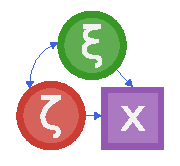
\includegraphics[width=.2\textwidth]{figures/logo_blue.pdf} \hspace{0.22cm}}
\newcommand{\nologo}{\setbeamertemplate{logo}{}} % command to set the logo to nothing
\nologo
\definecolor{mypurple}{RGB}{149, 88, 178}
\newcommand{\monob}[1]{\mbox{\texttt{\textcolor{mypurple}{#1}}}}

\newenvironment{wideitemize}{
    \itemize\addtolength{\itemsep}{15pt}\addtolength{\topsep}{10pt}}{\enditemize}

\newcommand{\A}{\mathbf{A}}
\newcommand{\I}{\mathbf{I}}
\newcommand{\F}{\mathbf{F}}
\newcommand{\OmegaM}{\mathbf{\Omega}}
\newcommand{\SigmaM}{\mathbf{\Sigma}}

\DeclareMathOperator{\prox}{prox}
\DeclareMathOperator*{\argmin}{arg\,min}

\begin{document}
	\setcounter{showProgressBar}{0}
	\setcounter{showSlideNumbers}{0}

	{
	\setbeamertemplate{background}{}
	\setbeamercolor{background canvas}{bg=ExecusharesWhite}
%     \begin{frame}
%         \centering
%         \setstretch{1.5}
%         With every wrinkled face, she sees a story untold, \\
%         Of a life full of laughter, love, and tears, hot and cold, \\
%         She listens with care, to the wisdom they share, \\
%         And learns about the paths that brought them there.\\
%         \hfill \\
%         ChatGPT  \\ (a poem about a PhD candidate in lifespan psychology)
%     \end{frame}
    }

    {
    %\setbeamertemplate{background}{}
	\frame{
	\titlepage}
	}

	%\setcounter{framenumber}{0}
	\setcounter{showProgressBar}{0}
	\setcounter{showSlideNumbers}{0}

	\section{Recap}

    \begin{frame}
    \frametitle{Recap}
        \begin{wideitemize}
            \item Workflow
            \item Syntax
            \item Types
            \item Multiple dispatch
        \end{wideitemize}
    \end{frame}

    \begin{frame}
    \frametitle{Types + Multiple Dispatch}
    You have \ldots
    \vspace{1cm}
        \begin{wideitemize}
            \item implemented linear regression
            \item implemented the Measurement type
            \item implemented methods for the Measurement type
        \end{wideitemize}
    \vspace{1cm}
    %while implementing linear regression, you did not know anything about Julia's type system
    %while define your measurement type, you did not have to know how linear regression works
    $\rightarrow$ Used it \textbf{together}\\
    \end{frame}

    \begin{frame}
    \frametitle{Types + Multiple Dispatch}
    \vspace{1cm}
        \begin{wideitemize}
            \item functions are composed of other functions
            \item if I can provide the relevant methods for my type, existing code also works for me
        \end{wideitemize}
        \vspace{1cm}
    \end{frame}

    \begin{frame}
    \frametitle{Types + Multiple Dispatch}
    \vspace{1cm}
        \begin{wideitemize}
            \item writing generic code gives you \textbf{extensibility for free} (and is \textbf{fast})
            \item altering the behaviour of \textbf{existing code} gives extensibility (without understanding it in detail)
        \end{wideitemize}
    \end{frame}

%     \begin{frame}
%     \frametitle{Why Julia? - the bottom line}
%     Because functions can implement everything you need, this mode of extensibility is widely applicable:
%     \vspace{1cm}
%         \begin{wideitemize}
%             \item there can be packages that work with flowers, spaceships or loss functions
%             \item that depends on the scent, speed or gradient
%             \item If I can add a new type and write the appropriate methods, it will work for me!
%         \end{wideitemize}
%     \end{frame}

    \section{Second Half}

    \begin{frame}
    \frametitle{Second Half}
    \vspace{1cm}
        \begin{wideitemize}
            \item break
            \item work on a topic that is interesting to you (in groups)
            \item brainstorm to find topics
            \item feedback
        \end{wideitemize}
    \end{frame}

	\section{Questions?}
\end{document}
